\section{modelling}


\subsection{overview}

Here we present the design- and interface details of the OMNeT-module 
\h{\bp}\footnote{We denote a Layer in a general meaning by 'physical layer' or
 'MAC layer' and our concrete C++ classes
by \h{\bp} or \h{\bm}.} to meet the requirement specification. That includes:

\begin{enumerate}
 \item internal class diagram of \h{\bp} and relation to \h{\bm}
 \item interface description for all involved C++ classes
 \item flow charts for reception of MacPacket from upper layer and 
 AirFrame from the channel
 \item some detailed flow charts for important sub processes
\end{enumerate}


\subsection{classgraph}

We start with the classgraph for the OMNeT-module \h{\bp} that shows its C++ classes,
 relations to other OMNeT-modules (especially \h{\bm})
and the OMNeT-messages sent between them.\\

The \h{\bp} holds a list\req{defanalogueMulti} of AnalogueModels and a pointer
to a
Decider. Thus the AnalogueModel and the Decider are submodules of \h{\bp}. This
way one is able to change\req{defanalogueExtensible}\req{defdeciderExtensible}
and
replace\req{defanalogueIndependent}\req{defdeciderIndependent} them
independently from
the \h{\bp}.

\begin{landscape}
\begin{figure}
 \centering
 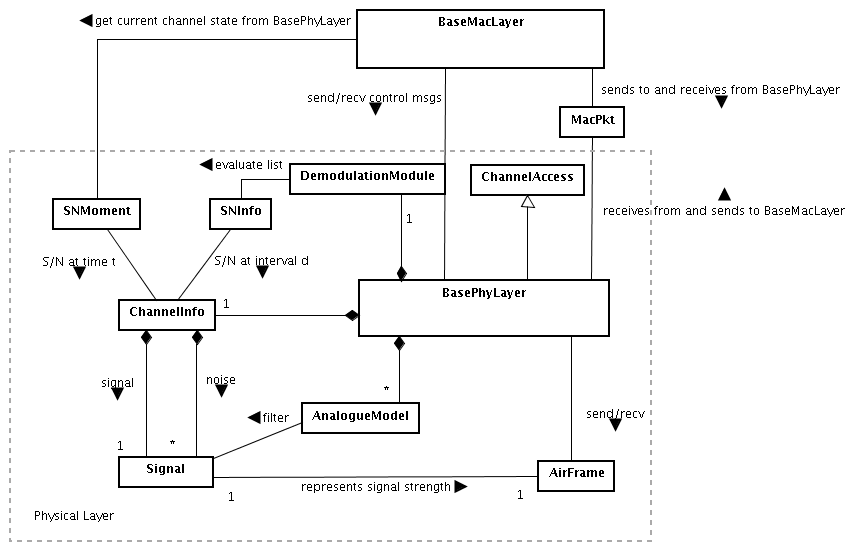
\includegraphics[width=21cm]{modelling/class_diagram.png}
 \caption{class graph}
 \label{fig: classgraph}
\end{figure}
\end{landscape} 

\subsection{The \bp}

In this section we focus on the module \h{\bp} and how one is able to communicate with the 
it, i.e. especially the \h{\bm} which is connected to the \h{\bp}
in three ways:

\begin{enumerate}
 \item OMNeT-channel for data messages
 \item OMNeT-channel for control messages
 \item a reference to the \h{MacToPhyInterface}.
\end{enumerate} 

The \underline{data channel} is used to send and receive\req{defpacketFromMac}
MacPkts to and
from the \h{\bp}. An appropriate ControlInfo is attached to the packet by the
sending layer. The \h{MacToPhyControlInfo} is the carrier of the Signal from the
MAC-Layer down to the Physical-Layer.
\saf{MacToPhyCtrlInfo interface}\\

The \underline{control channel} is used by the \h{\bp} to inform the \h{\bm}
about
certain events\req{defprovactive}, e.g. the TX\_OVER\req{deftxover} message 
which indicates the end of a sending transmission.

A ChannelSenseRequest can be sent over \underline{control channel} from \h{\bm}
to \h{\bp}. It is handed to the Decider (several times) that attaches a
ChannelState and finally sent back to \h{\bm}.
\begin{figure}[H]
 \centering
 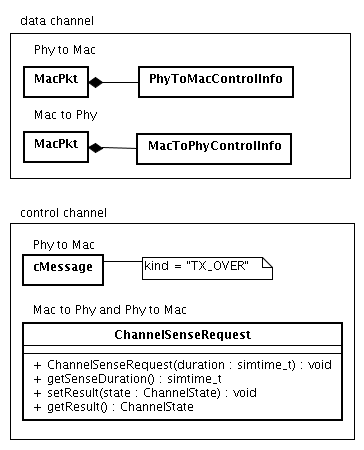
\includegraphics[width = 0.7\textwidth]{modelling/PhyMacMessages.png}
 \caption{messages sent between \h{\bp} an \h{\bm}}
 \label{fig: PhyMacMessages}
\end{figure}


The \underline{reference} provides a passive way\req{defprovpassive} for the  \h{\bm} to 
get
information about the current channel state\req{defchannelstate} (that is an
alternative [immediate answer] to sending a ChannelSenseRequest) and to
get\req{defcurrentmode} and set\req{defswitchmode} the current radiostate (RX,
TX,
SLEEP).
Switching times\req{defswitchtimes} from one radio state to another are
controlled
internally by a state machine. \saf{mode state machine} and \ref{radio}
\\
This functionality offered to \h{\bm} beside OMNeT is defined by the \h{MacToPhyInterface}.
\\

Further the \h{\bp} has an interface \h{DeciderToPhyInterface} that defines the functionality
needed by the Decider. (see also \ref{decider})
% interface description here
\label{SignalCreation}

\begin{figure}[H]
 \centering
 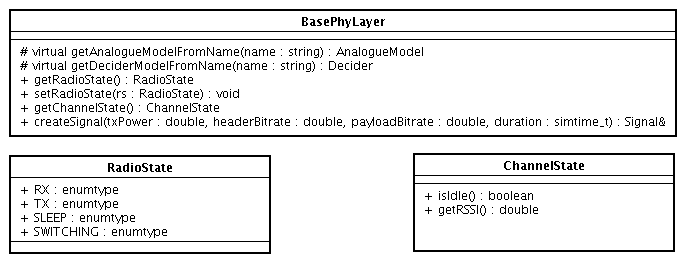
\includegraphics[width = \textwidth]{modelling/BasePhyLayer_members.png}
 \caption{BasePhyLayer interface}
 \label{fig: BasePhyLayer interface}
\end{figure}

\begin{figure}[H]
 \centering
 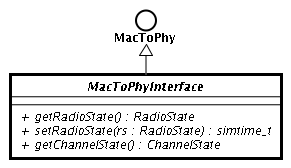
\includegraphics{modelling/MacToPhyInterface_members.png}
 \caption{MacToPhy interface}
 \label{fig: The MacToPhyInterface}
\end{figure}

\subsection{Radio}
\label{radio}

The Radio-class implements the radio of the host as a state machine under supervision
of the \h{\bp}. Instructions from \h{\bm} concerning the radio are handled by \h{\bp}.

\begin{figure}[H]
 \centering
 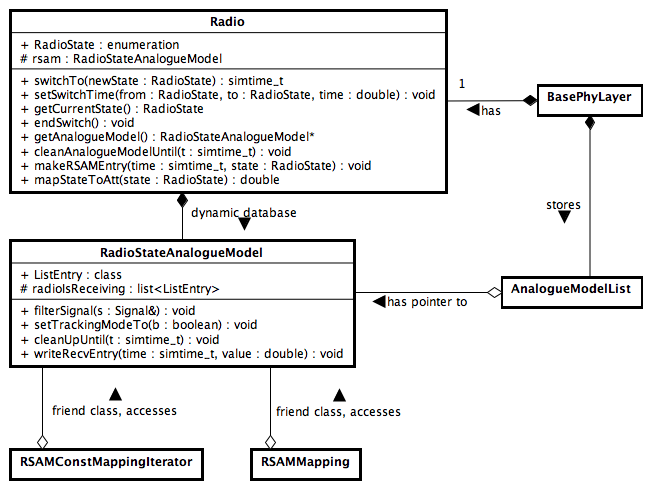
\includegraphics[width = \textwidth]{modelling/Radio_detail.png}
 \caption{The Radio class}
 \label{fig: radio}
\end{figure}

\subsection{AnalogueModel}
%\label{AM and Signal}

%The Signal is designed one-dimensional (power-over-time) by default with a
%specified time point for start and end of the Signal. The owner is able
%to add and request values at a specific time point\req{defsendInfoTXPower}.
%The Method getTimeIterator() returns an appropriate SignalTimeIterator needed
%for applying AnalogueModels to the Signal.

%\begin{quote}
%\emph{NOTE: Anyone who subclasses Signal should make shure to have a properly
%working SignalTimeIterator (subclassed) for it. The SignalTimeIterator should
%always iterate over every time stamp in each dimension. This way simple
%AnalogueModels will be able to filter the Signal independent from its
%dimension.}
%\end{quote}

%Further the Signal is set the packets bitrate over
%time\req{defsendInfoBitrate}, 
%the Move of the Host\req{defsendInfoMove}, the size of the
%packet\req{defsendInfoSize} and the channel dimensions\req{defsendInfoChannel}
%by
%\h{\bp}.
%
%\emph{See also \ref{AirFrame and Signal}.}

The AnalogueModel is at least able to filter the \emph{TX-Power over
time}-Signal.\\

Information how it works on a more complex multi-dimensional Signal are
explained in section \ref{sec:signaldetail}.
 
\begin{figure}[H]
 \centering
 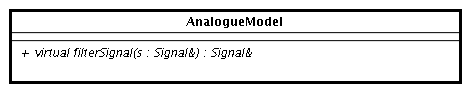
\includegraphics[width = \textwidth]{modelling/AnalogueModel_members.png}
 \caption{analogue model interface}
 \label{fig: analogue model interface}
\end{figure}
%
%The AnalogueModel offers functionality to filter a referenced
%signal\req{defanalogueFilter} in a specified interval\req{defrcvFilterSignals}
%(e.g.
%preamble\req{defrcvFilterPreamble}) or at a single point in time.

%Three basic AnalogueModel classes are foreseen to be plugged into Phy-Layer to
%simulate pathloss\req{defanalogueSimPathloss},
%shadowing\req{defanalogueSimShadowing}
%and fading\req{defanalogueSimFading}.\\
%\h{\bp} is designed to apply an arbitrary number of AnalogueModels to a Signal.

% \begin{figure}[H]
%  \centering
%  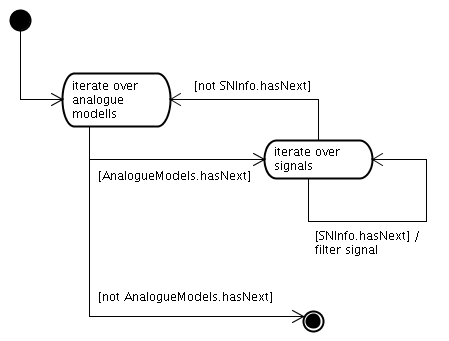
\includegraphics[width =
%0.8\textwidth]{modelling/apply_analogue_modells_detail.png}%[width=300pt]
%  \caption{application of analogue models}
%  \label{fig: application analogue models}
% \end{figure}



\subsection{ChannelInfo}

ChannelInfo keeps track of all AirFrames on the channel. It does not
differentiate between \textit{signal} and \textit{noise}. \h{\bp} is able to
add and remove references to certain AirFrames to and from ChannelInfo.\\
ChannelInfo can identify all AirFrames that intersect with a
given time interval and write them to an output-vector.

\begin{figure}[H]
 \centering
 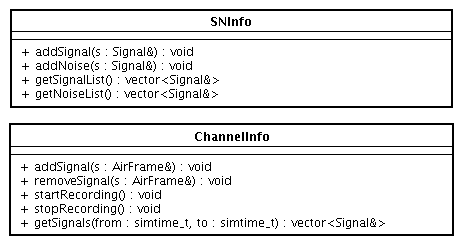
\includegraphics[width = \textwidth]{modelling/ChannelInfo_members.png}
 \caption{channel details}
 \label{fig: channel details}
\end{figure}
